%%%%%%%%%%%%%%%%%%%%%%%%%%%%%%%%%%%%%%%%%
% Dreuw & Deselaer's Poster
% LaTeX Template
% Version 1.0 (11/04/13)
%
% Created by:
% Philippe Dreuw and Thomas Deselaers
% http://www-i6.informatik.rwth-aachen.de/~dreuw/latexbeamerposter.php
%
% This template has been downloaded from:
% http://www.LaTeXTemplates.com
%
% License:
% CC BY-NC-SA 3.0 (http://creativecommons.org/licenses/by-nc-sa/3.0/)
%
%%%%%%%%%%%%%%%%%%%%%%%%%%%%%%%%%%%%%%%%%

%----------------------------------------------------------------------------------------
%	PACKAGES AND OTHER DOCUMENT CONFIGURATIONS
%----------------------------------------------------------------------------------------

\documentclass[final]{beamer}

\usepackage[orientation=portrait,size=a0,scale=1.45]{beamerposter} 
% Use the beamerposter package for laying out the poster with a 
% portrait orientation and an a0 paper size

\usetheme{I6pd2} % Use the I6pd2 theme supplied with this template

\usepackage[english]{babel} % English language/hyphenation
\usepackage{ragged2e} %to use justify
\usepackage{amsmath,amsthm,amssymb,latexsym} % For including math 
% equations, theorems, symbols, etc
\usepackage{epstopdf}
%\usepackage{times}\usefonttheme{professionalfonts}  % Uncomment to use 
%\usefonttheme{professionalfonts} % using non standard fonts for beamer
%\usefonttheme{serif} % default family is serif
%\usepackage{fontspec}
%\setmainfont{Liberation Serif}
% Times as the main font
%\usefonttheme[onlymath]{serif} % Uncomment to use a Serif font within 
% math environments
\usepackage{multicol}

%\boldmath % Use bold for everything within the math environment

\usepackage{booktabs} % Top and bottom rules for tables
\usepackage{graphicx}
\usepackage{multirow}
\usepackage{gensymb}
\usepackage{float}
\usepackage{MnSymbol}
\usepackage{gensymb}
\usepackage{wrapfig}
%\usepackage[final]{graphicx}
\graphicspath{{figures/}} % Location of the graphics files

\usecaptiontemplate{\small\structure{\insertcaptionname~\insertcaptionnumber: }\insertcaption} % A fix for figure numbering


\usepackage{xstring}

\setbeamertemplate{block begin}
{
  \par\vskip\medskipamount%
  \IfStrEq{\insertblocktitle}{}{}{
      \begin{beamercolorbox}[colsep*=.75ex]{block title}
        \usebeamerfont*{block title}\insertblocktitle%
      \end{beamercolorbox}%
  }
  {\parskip0pt\par}%
  \ifbeamercolorempty[bg]{block title}
  {}
  {\ifbeamercolorempty[bg]{block body}{}{\nointerlineskip\vskip-0.5pt}}%
  \usebeamerfont{block body}%
  \begin{beamercolorbox}[colsep*=.75ex,vmode]{block body}%
    \ifbeamercolorempty[bg]{block body}{\vskip-.25ex}{\vskip-.75ex}\vbox{}%
}



%----------------------------------------------------------------------------------------
%	TITLE SECTION 
%----------------------------------------------------------------------------------------

\title{\Huge Ionization of biological molecules by multicharged ions} 

\author{\Large 
 A M P Mendez, %\writeto{alemendez@iafe.uba.ar},
 C C Montanari,
 and J E Miraglia
}

\institute{Instituto de Astronom\'{\i}a y F\'{\i}sica del Espacio, CONICET--UBA}


%----------------------------------------------------------------------------------------
%	FOOTER TEXT
%----------------------------------------------------------------------------------------

\newcommand{\leftfoot}{}%http://www.LaTeXTemplates.com} 
% Left footer text

\newcommand{\rightfoot}{$^*$ alemendez@iafe.uba.ar} 
% Right footer text

%%%%%%%%%%%%%%%%%%%%%%%%%%%%%%%%%%%%%%%%%%%%%%%%%%%%%%%%%%%%%%%%%%%%%%%%%
%%%%%%%%%%%%%%%%%%%%%%%%%%%%%%%%%%%%%%%%%%%%%%%%%%%%%%%%%%%%%%%%%%%%%%%%%
%%%%%%%%%%%%%%%%%%%%%%%%%%%%%%%%%%%%%%%%%%%%%%%%%%%%%%%%%%%%%%%%%%%%%%%%%

\begin{document}

\addtobeamertemplate{block end}{}{\vspace*{2ex}} 
% White space under blocks

\begin{frame}[t] 
%%%%%%%%%%%%%%%%%%%%%%%%%%%%%%%%%%%%%%%%%%%%%%%%%%%%%%%%%%%%%%%%%%%%%%%%%
\begin{columns}[t] 
\begin{column}{.03\textwidth}
\end{column} % Empty spacer column
\begin{column}{.46\textwidth} % The first column
\vspace{-5mm}
%------------------------------------------------------------------------
%	INTRODUCTION
%------------------------------------------------------------------------
\begin{block}{Introduction}
\justify

The \colorbox{tabutter}{ionization of biological targets} by the impact of heavy projectiles 
has become a field of interest due to its implementation in ion-beam 
cancer therapy. The study of such systems represents a challenge from 
the theoretical point of view; however, several approaches 
\cite{galassi2000,ludde2016} have been presented to deal with this process. 

We investigate the ionization of several biological molecules of 
interest by the impact of multicharged ions in the 
\colorbox{tabutter}{intermediate to high energy range} using the Continuum 
Distorted Wave-Eikonal Initial State
method (CDW)~\cite{fainstein1988} and the simple stoichiometric 
model (SSM)~\cite{mendez2019}. 

\vspace{0.5cm}

\end{block}
%------------------------------------------------------------------------
%	ATOMS
%------------------------------------------------------------------------
\begin{block}{Ionization of atoms}
\justify

\vspace{1.cm}
\begin{minipage}{\textwidth}
\begin{columns}[T]
\begin{column}{0.025\textwidth}
\end{column}
\begin{column}{0.8\textwidth}
We considered 36 collisional systems composed by 
\begin{itemize}
\item targets: $\alpha=$ \colorbox{tabutter}{H, C, N, O, P, and S,}
\item projectiles: \colorbox{tabutter}{$\bar{p}$, H$^{+}$, He$^{2+}$, Be$^{4+}$, C$^{6+}$, and O$^{8+}$.}
\end{itemize}
The total ionization cross section was calculated using the 
CDW~\cite{miraglia2019}.
\end{column}
\begin{column}{0.2\textwidth}
\includegraphics[width=6cm]{miraglia2019.eps}
\end{column}
\end{columns}
\end{minipage}

\vspace{0.1cm}
\begin{figure}
\centering
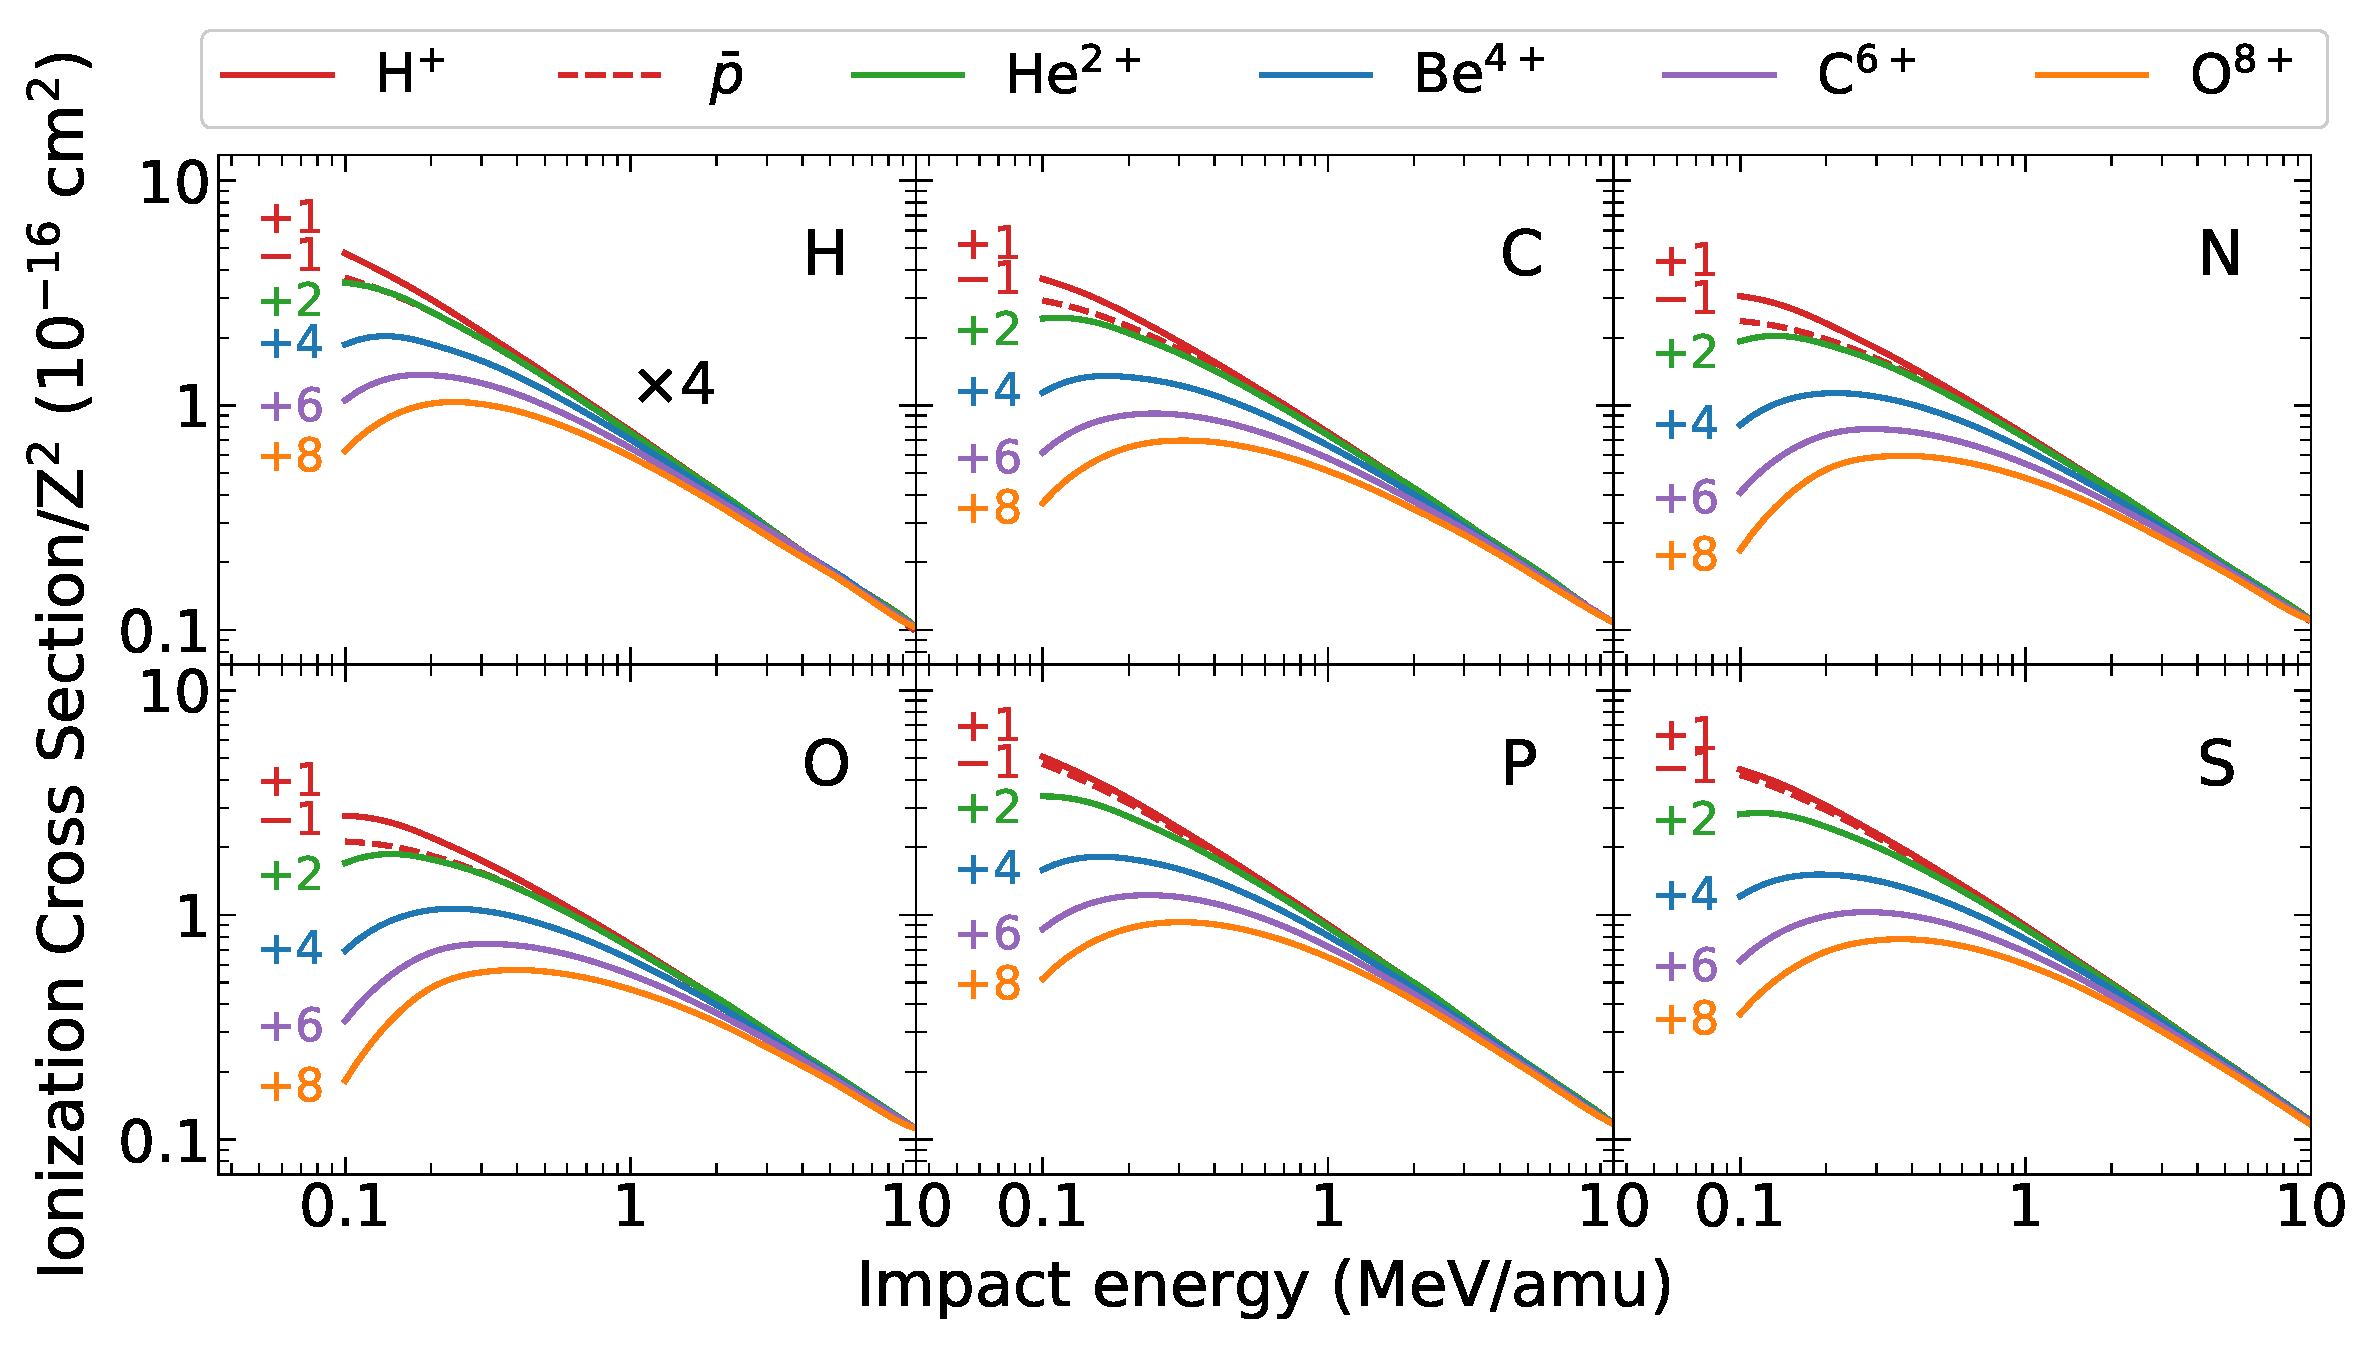
\includegraphics[width=0.95\textwidth]{figures/atomicscaling.eps}
\end{figure}

\end{block}
%------------------------------------------------------------------------
%	NEW SCALING
%------------------------------------------------------------------------
\begin{block}{Scaling rules}
\justify

Following~\cite{toburen1975}, we define the scaled ionization cross 
section per weakly bound electron $\sigma_{e}$ as
\begin{equation}
\sigma_e=\frac{\sigma_M}{n_e}\,, 
\end{equation}
where $n_e=\sum_{\alpha}n_{\alpha}\nu_{\alpha}$, and $\nu_{\alpha}$ 
are the active electron numbers given by
\begin{equation}
\nu_{\alpha}=\left\{ 
\begin{array}{lcll}
1, & \rightarrow & 1 & \text{for H,} \\
4, & \rightarrow &  4 & \text{for C,} \\ 
5, & \rightarrow &  4 & \text{for N and P,} \\ 
6, & \rightarrow &  4.5 & \text{for O and S}\,.
\end{array}\right.
\label{eq:nelec} 
\end{equation} 

\vspace{-1cm}
\begin{figure}
\centering
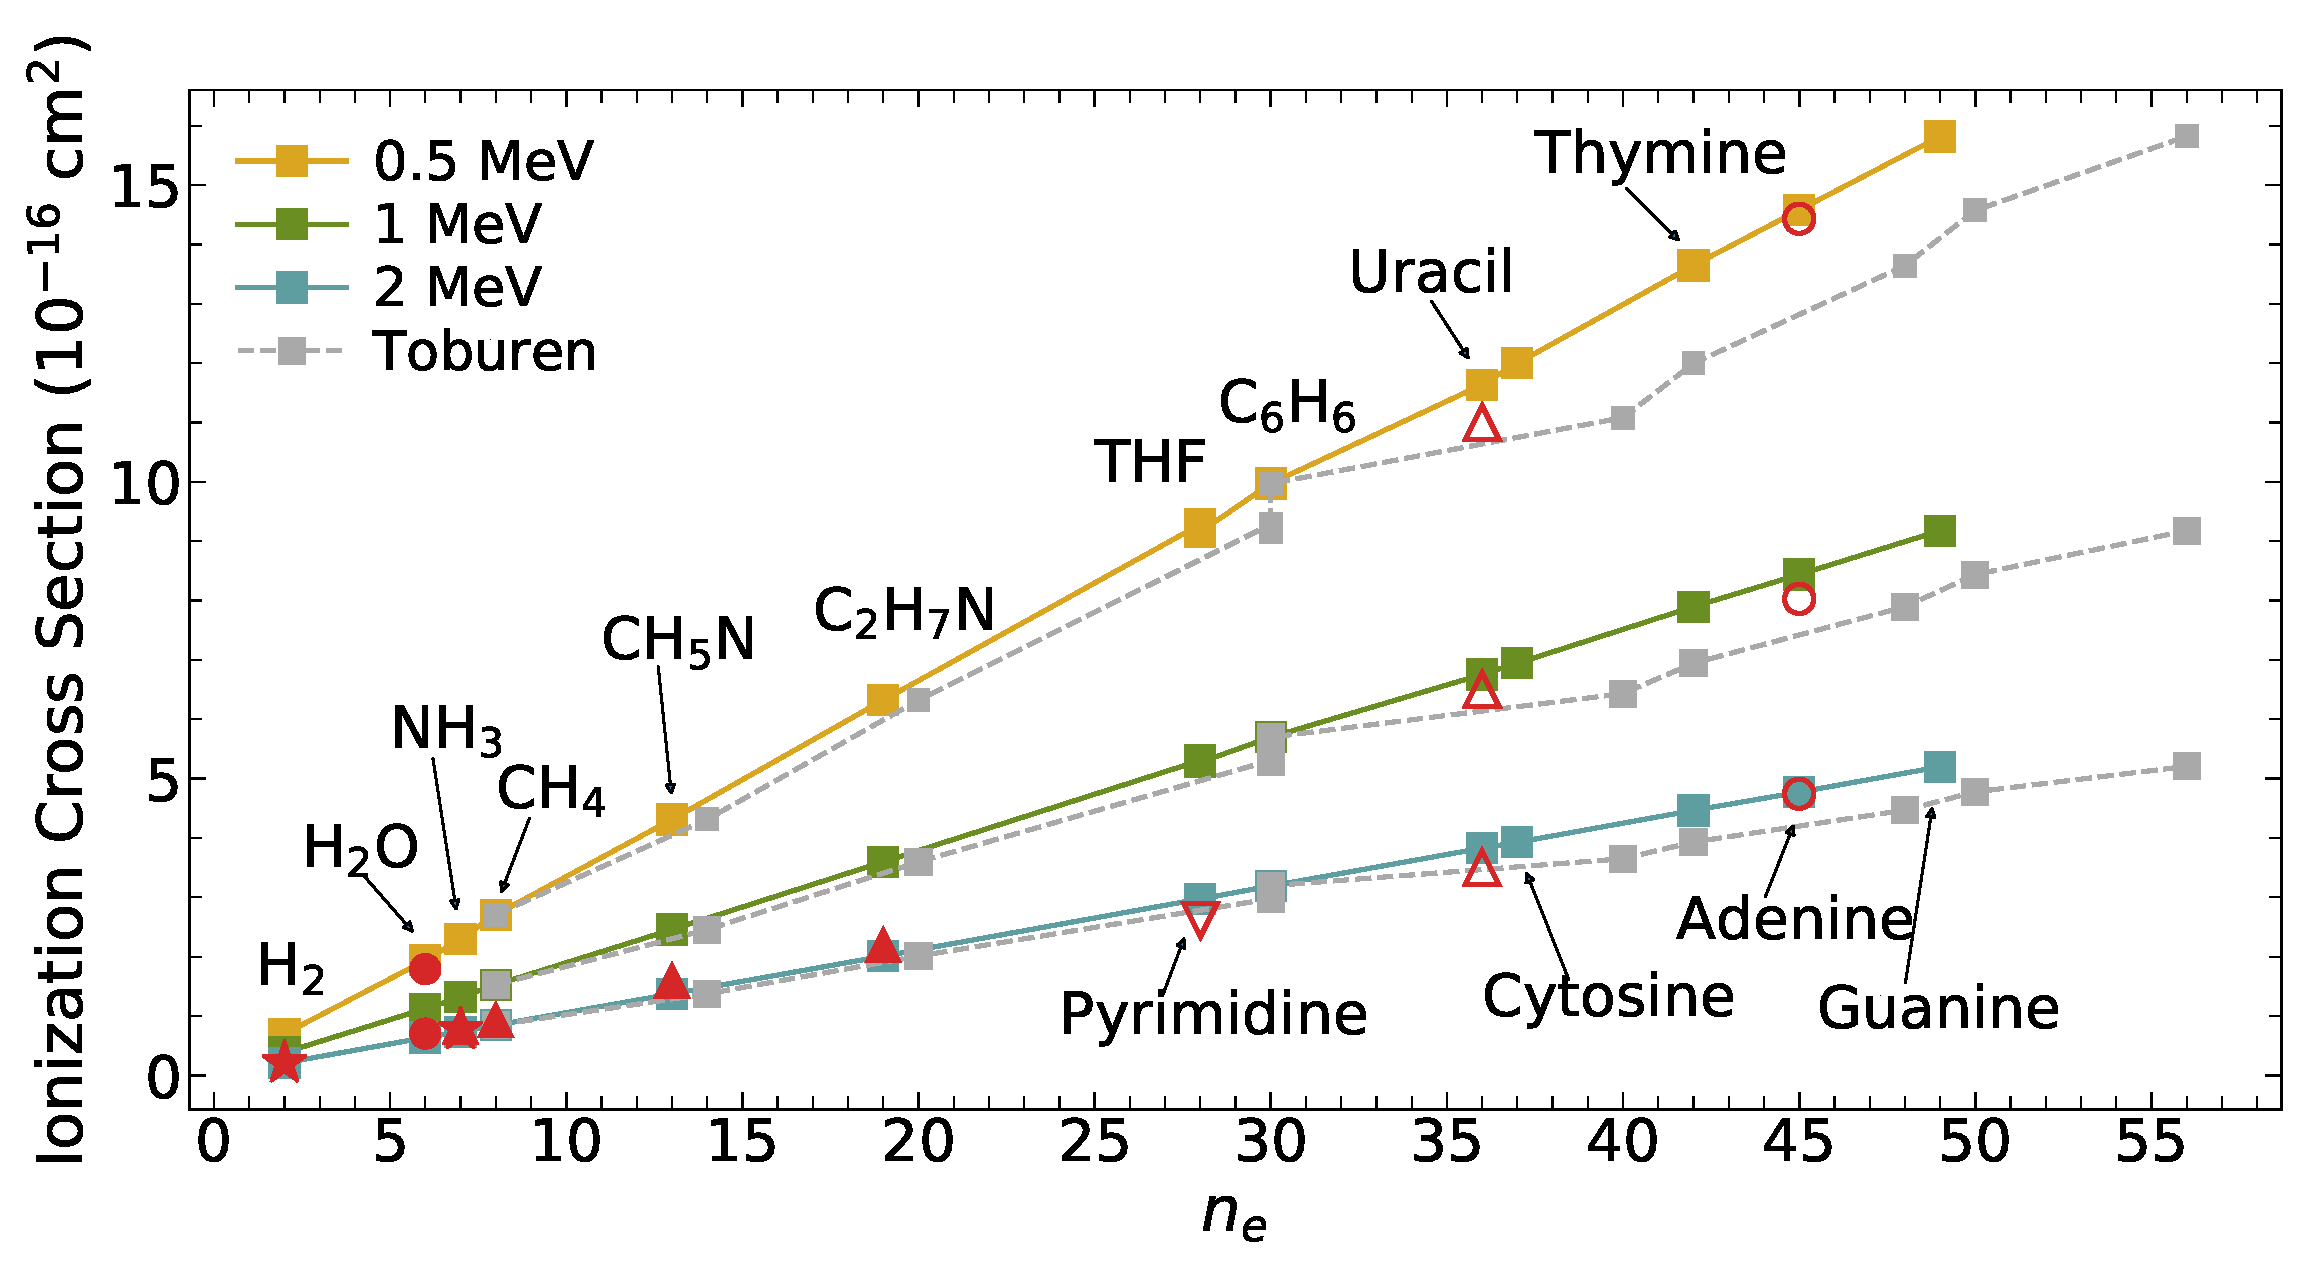
\includegraphics[width=0.9\textwidth]{figures/scale_ne.eps}
\end{figure}

\end{block}
%%%%%%%%%%%%%%%%%%%%%%%%%%%%%%%%%%%%%%%%%%%%%%%%%%%%%%%%%%%%%%%%%%%%%%
\setbeamercolor{block title}{fg=black,bg=orange!70} 
% Change the block title color
\end{column} % End of the first column
\begin{column}{.02\textwidth}
\end{column} % Empty spacer column
\begin{column}{.44\textwidth} % The second column
%%%%%%%%%%%%%%%%%%%%%%%%%%%%%%%%%%%%%%%%%%%%%%%%%%%%%%%%%%%%%%%%%%%%%%
%------------------------------------------------------------------------
%	STOICHIOMETRIC MODEL
%------------------------------------------------------------------------
\begin{block}{The stoichiometric model}
\justify

The SSM approaches the total ionization cross 
section of a molecule $M$ as
\begin{equation}
 \sigma_{M}=\sum\limits_{\alpha}n_{\alpha}\sigma_{\alpha}\,.  
\end{equation}
where $n_{\alpha}$ is the number of element $\alpha$ forming the molecule
and $\sigma_{\alpha}$ is the ionization cross sections 
of the isolated atoms.
\end{block}

%------------------------------------------------------------------------
%	STOICHIOMETRIC MODEL
%------------------------------------------------------------------------
\begin{block}{Molecules studied}
\justify
We considered the following molecules:
\begin{itemize}
\item CH: \hspace{0.45cm} CH$_4$, C$_2$H$_2$, C$_2$H$_4$, C$_2$H$_6$, C$_6$H$_6$ \\
\item CHN: C$_5$H$_5$N, C$_4$H$_4$N$_2$, C$_2$H$_7$N, CH$_5$N \\
\item DNA: C$_5$H$_5$N$_5$, C$_4$H$_5$N$_3$O, C$_5$H$_5$N$_5$O, C$_5$H$_6$N$_2$O$_2$, C$_4$H$_4$N$_2$O$_2$, 
\\ \hspace{2.85cm} C$_4$H$_8$O, C$_5$H$_{10}$O$_5$P, C$_{20}$H$_{27}$N$_7$O$_{13}$P$_2$ 
\end{itemize}

\end{block}
%------------------------------------------------------------------------
%	DNA AND RNA BASES
%------------------------------------------------------------------------
\begin{block}{Ionization of DNA and RNA bases}
\justify

\begin{figure}
\centering
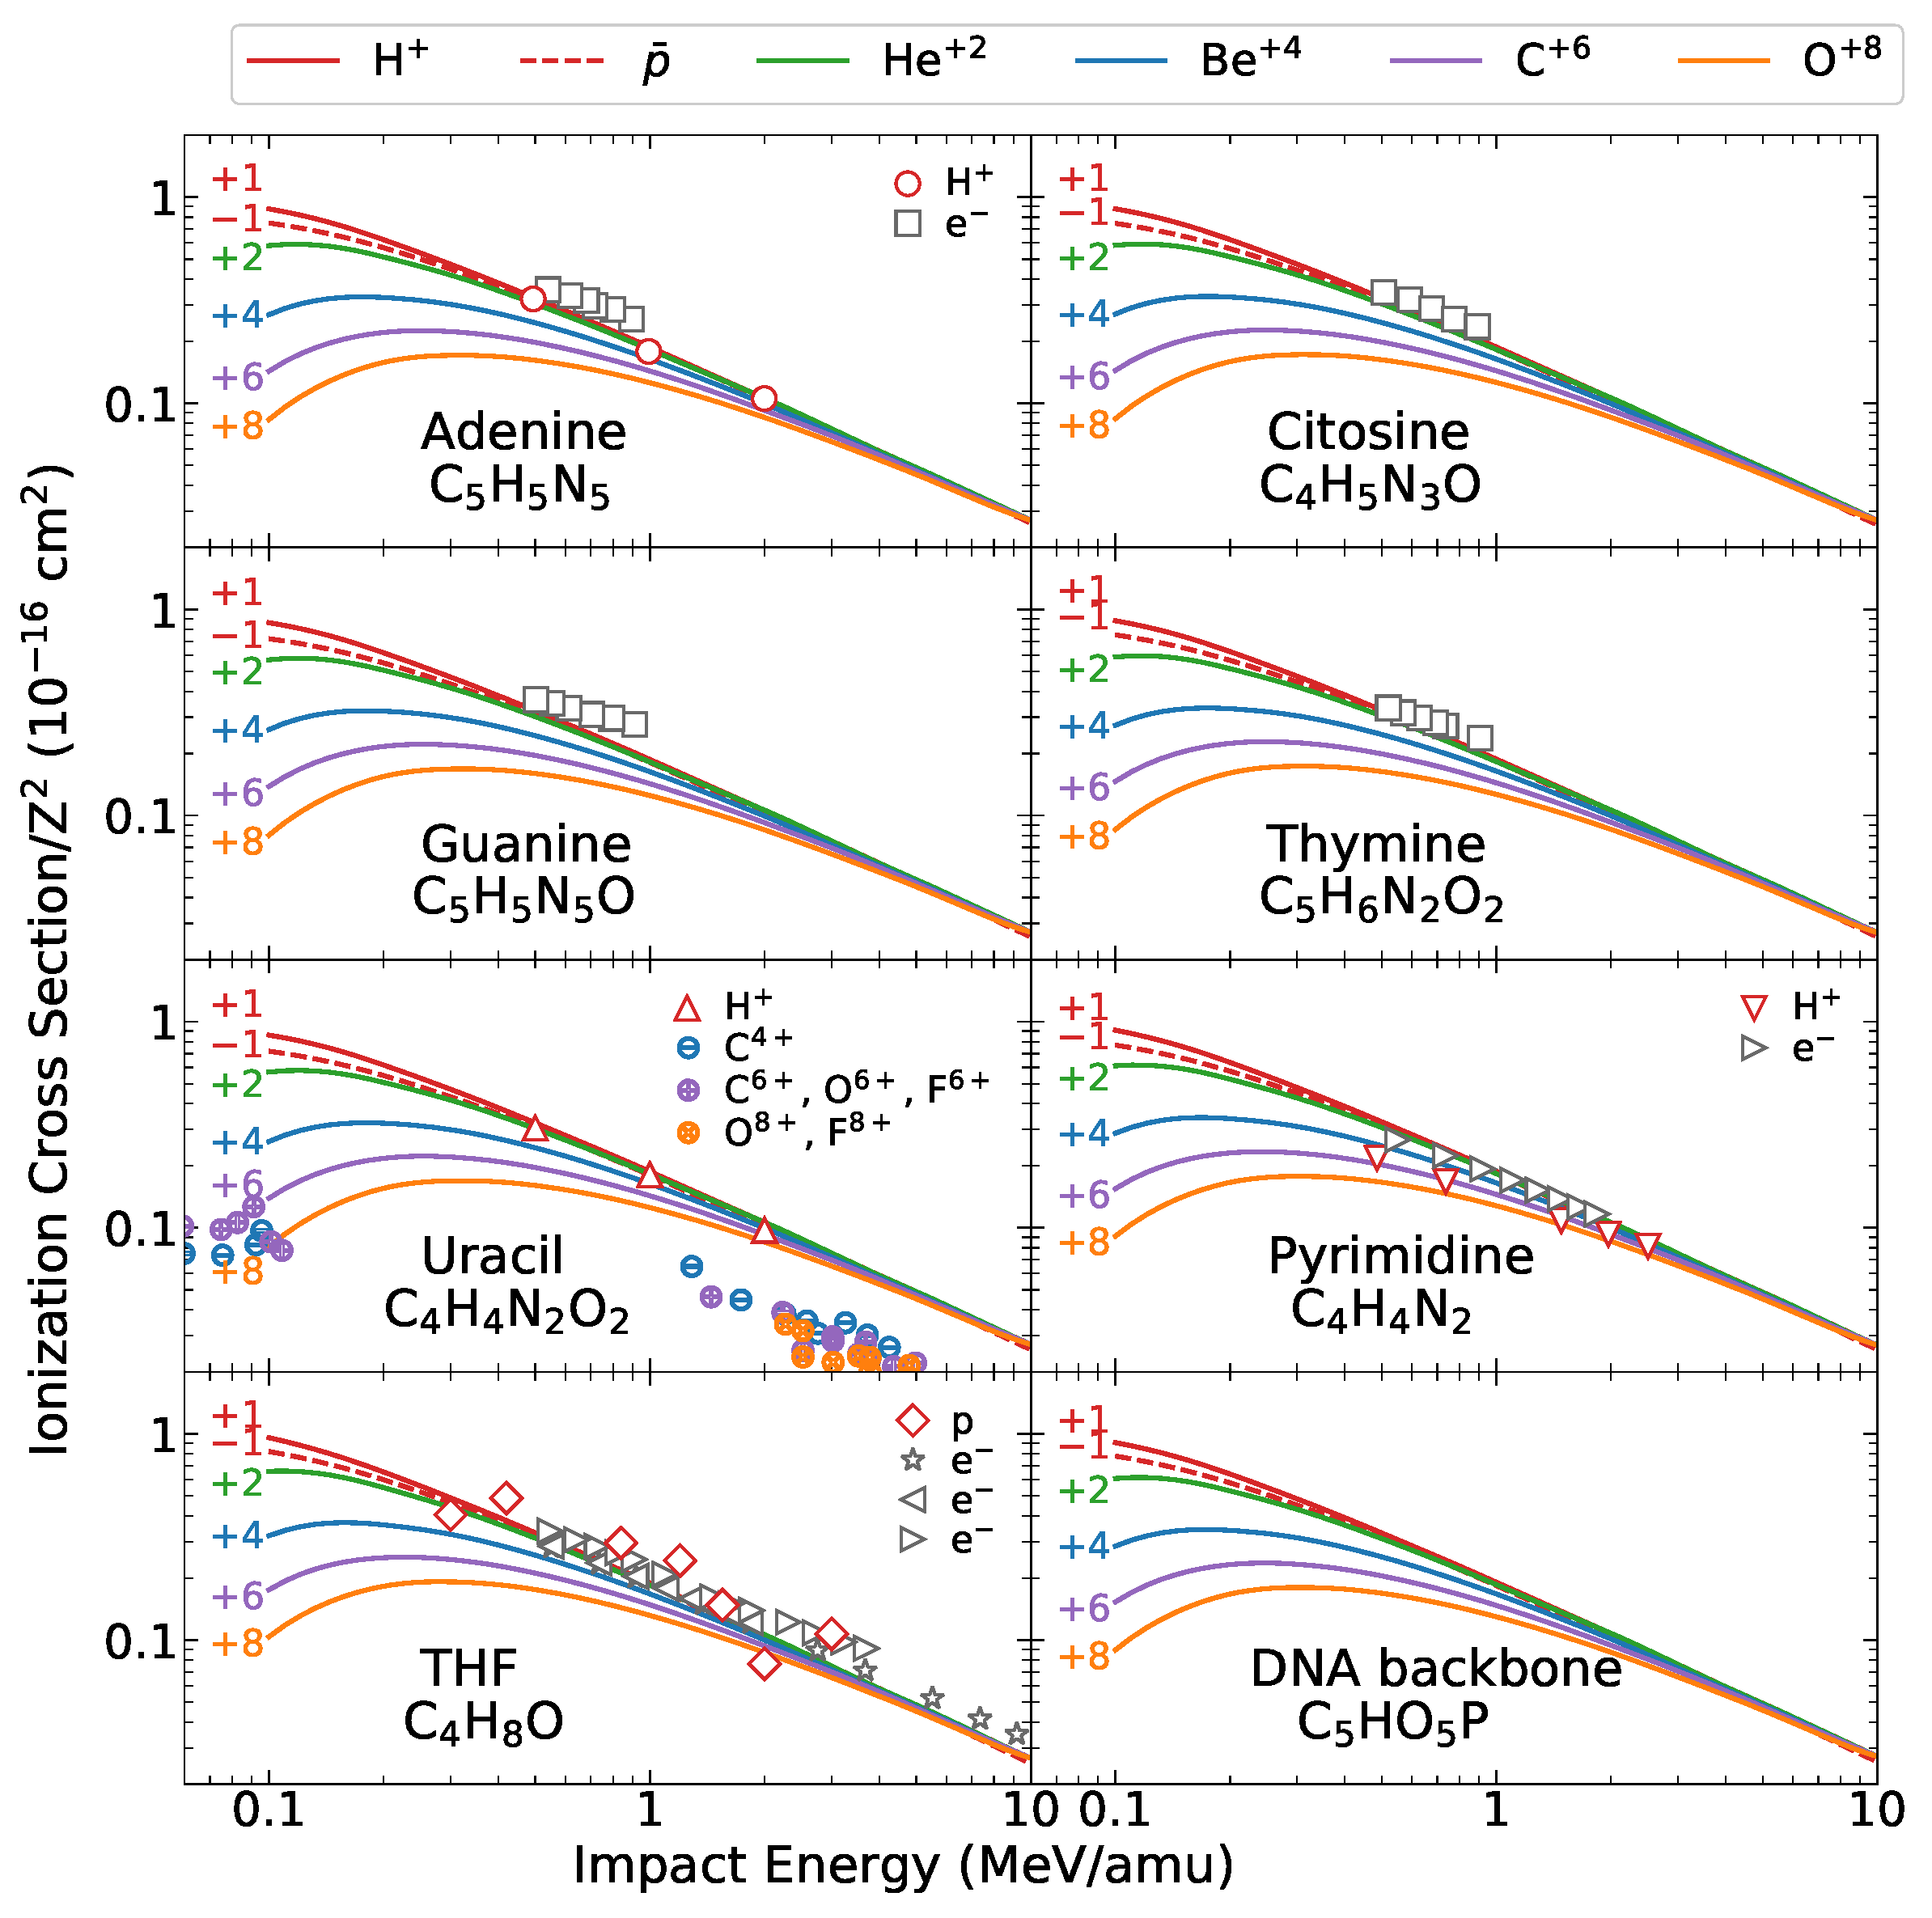
\includegraphics[width=0.95\textwidth]{figures/adn_all.eps} 
\end{figure}

\end{block}
%------------------------------------------------------------------------
%	NEW SCALING
%------------------------------------------------------------------------
\begin{block}{CDW--based scaling}
\justify

\begin{figure}
\centering
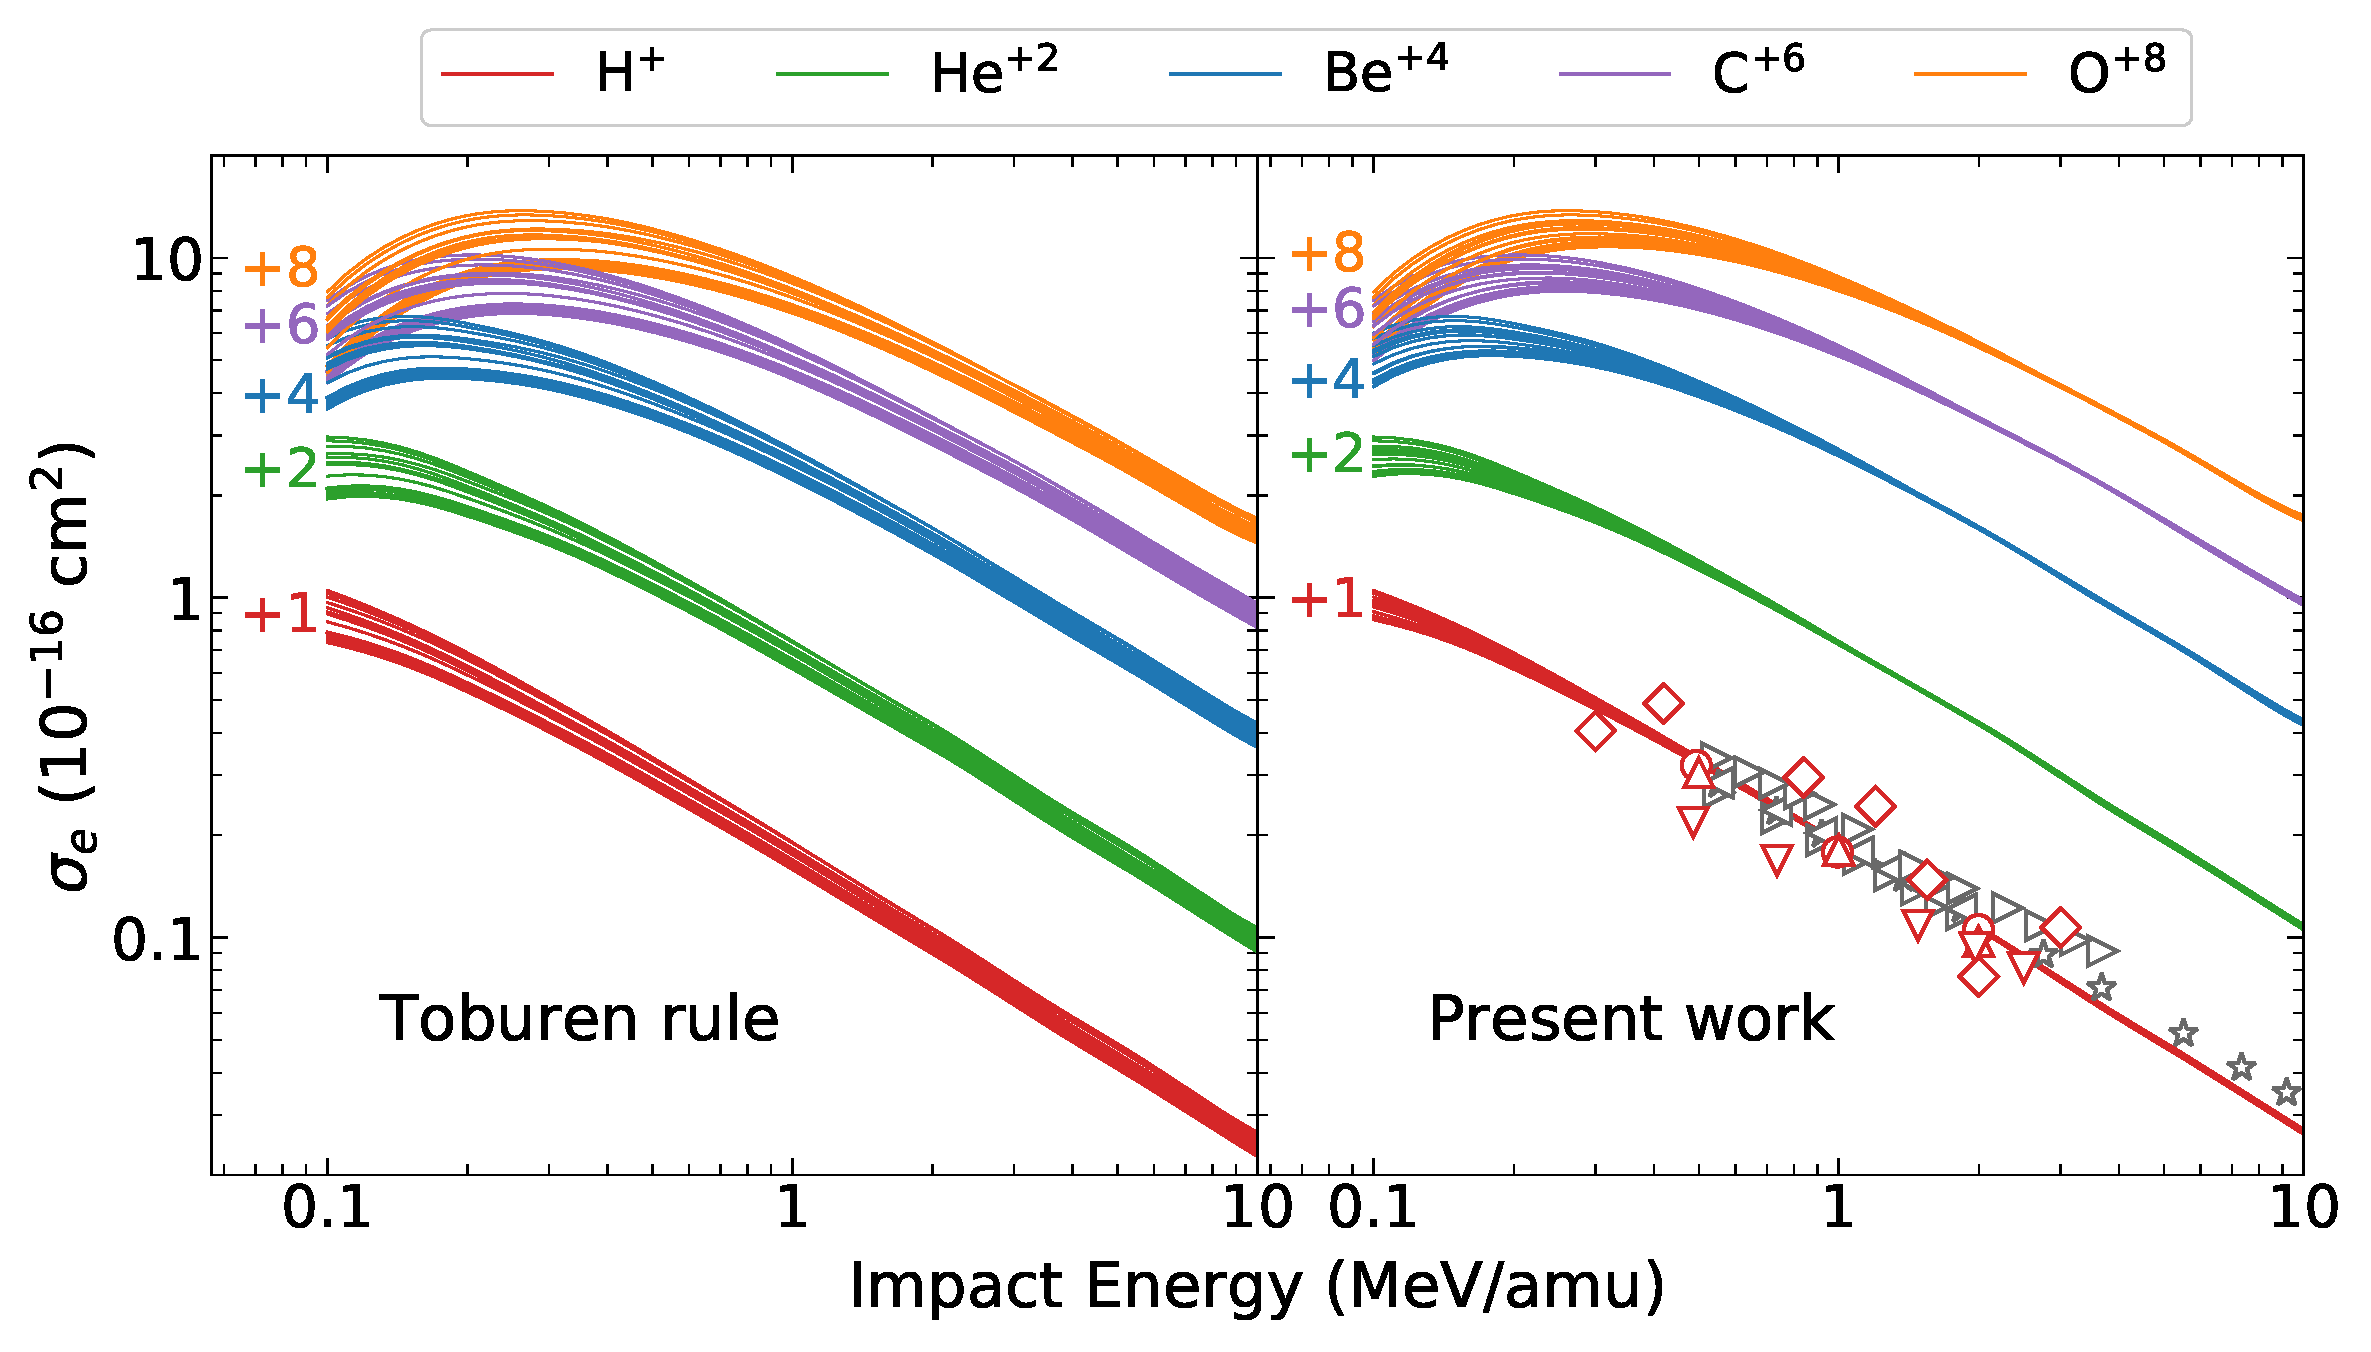
\includegraphics[width=0.98\textwidth]{figures/molscaling85.eps} 
\end{figure}

\end{block}
%%%%%%%%%%%%%%%%%%%%%%%%%%%%%%%%%%%%%%%%%%%%%%%%%%%%%%%%%%%%%%%%%%%%%%%%%
%%%%%%%%%%%%%%%%%%%%%%%%%%%%%%%%%%%%%%%%%%%%%%%%%%%%%%%%%%%%%%%%%%%%%%%%%
\end{column} % End of the second column
\begin{column}{.02\textwidth}
\end{column} % Empty spacer column
\end{columns} % End of all the columns in the poster
%%%%%%%%%%%%%%%%%%%%%%%%%%%%%%%%%%%%%%%%%%%%%%%%%%%%%%%%%%%%%%%%%%%%%%%%%
\begin{columns}[t] 
\begin{column}{.03\textwidth}
\end{column} % Empty spacer column
\begin{column}{.8\textwidth} 
%%%%%%%%%%%%%%%%%%%%%%%%%%%%%%%%%%%%%%%%%%%%%%%%%%%%%%%%%%%%%%%%%%%%%%%%%
%%%%%%%%%%%%%%%%%%%%%%%%%%%%%%%%%%%%%%%%%%%%%%%%%%%%%%%%%%%%%%%%%%%%%%%%%
%------------------------------------------------------------------------
%	REFERENCES
%------------------------------------------------------------------------
\begin{block}{References}

\vspace{-1.9cm}
\begin{multicols}{2}
\begin{thebibliography}{9}
 
\bibitem{galassi2000}
M. E. Galasssi, R. D. Rivarola, M. Beuve, G. H. Olivera and P. D. Fainstein, 
Phys. Rev. A \textbf{62}, 022701 (2000).

\vspace{-0.75cm}
\bibitem{ludde2016}
H. J. L\"udde, A. Achenbach, T. Kalkbrenner, H.-C. Jankowiak and T. Kirchner,
Eur. Phys. J. D \textbf{70}, 82 (2016).

\vspace{-0.75cm}
\bibitem{fainstein1988}
Fainstein P.D., Ponce V. H. and Rivarola R. D. 
J. Phys. B: At. Mol. Opt. Phys. \textbf{21} 287 (1988).

\vspace{-0.75cm}
\bibitem{mendez2019}
A. M. P. Mendez, C. C. Montanari and J. E. Miraglia,
arXiv:1909.13847 [physics.atm-clus]

\vspace{-0.75cm}
\bibitem{miraglia2019} 
J. E. Miraglia, 
https://arxiv.org/abs/1909.13682 [physics.atom-ph]

\vspace{-0.75cm}
\bibitem{toburen1975} 
W. E. Wilson and L. H. Toburen,
Phys. Rev. A \textbf{11}, 1303 (1975).

\end{thebibliography}
\end{multicols}
\vspace{-0.5cm}

\end{block}
%%%%%%%%%%%%%%%%%%%%%%%%%%%%%%%%%%%%%%%%%%%%%%%%%%%%%%%%%%%%%%%%%%%%%%%%%
%%%%%%%%%%%%%%%%%%%%%%%%%%%%%%%%%%%%%%%%%%%%%%%%%%%%%%%%%%%%%%%%%%%%%%%%%
\end{column}
\begin{column}{.14\textwidth} 

\begin{figure}
\includegraphics[width=0.95\textwidth]{mendez2019.eps}
\end{figure}

\end{column}
\begin{column}{.02\textwidth}
\end{column} % Empty spacer column
\end{columns} 
%%%%%%%%%%%%%%%%%%%%%%%%%%%%%%%%%%%%%%%%%%%%%%%%%%%%%%%%%%%%%%%%%%%%%%%%%
\end{frame} % End of the enclosing frame

\end{document}
%%%%%%%%%%%%%%%%%%%%%%%%%%%%%%%%%%%%%%%%%%%%%%%%%%%%%%%%%%%%%%%%%%%%%%%%%
